\documentclass{report}
\usepackage[utf8]{inputenc}
\usepackage{hyperref}
\usepackage{setspace}
\usepackage{float}
\title{Universal Parabolic Constant}

\author{Balakrishnan Rajagopal (40075977) }
\date{}
\renewcommand{\baselinestretch}{1.15}

\usepackage{natbib}
\usepackage{graphicx}

\usepackage[final]{pdfpages}


\usepackage{fancyhdr}
\usepackage[margin=1in]{geometry}
\usepackage{pdfpages}
\renewcommand{\headrulewidth}{0.1pt}
\fancyhf{} 
\renewcommand{\headrulewidth}{0.1pt} 
\fancyfoot[C]{\thepage} 
\renewcommand{\footrulewidth}{0.1pt} 


\begin{document}
\maketitle
\tableofcontents
\chapter{Universal Parabolic Constant}
\section{Description}
\onehalfspacing
The Universal parabolic constant is a mathematical constant and is defined as the ratio, for any parabola, of the arc length of the parabolic segment formed by the latus rectum to the focal parameter. The focal parameter is twice the focal length. The ratio is denoted P. Just as the ratio of the arc length of a semicircle to its radius is always pi, the ratio P of the arc length of the parabolic segment formed by the latus rectum of any parabola to its semilatus rectum (and focal parameter) is a universal constant. The other conic sections, namely the ellipse and hyperbola, do not have such universal constants because the analogous ratios for them depend on their eccentricities. In other words, all circles are similar and all parabolas are similar, but the same is not true for ellipses or hyperbolas.\newline
\newline The value of P is,

\begin{equation}
P = \ln(1+\sqrt{2})+\sqrt{2} = 2.29558714939
\end{equation}

\newline In the diagram (Fig 1), the latus rectum is pictured in blue, the parabolic segment that it forms in red
and the focal parameter in green. (The focus of the parabola is the point F and the directrix is the line L.)



\begin{figure}
\centering
    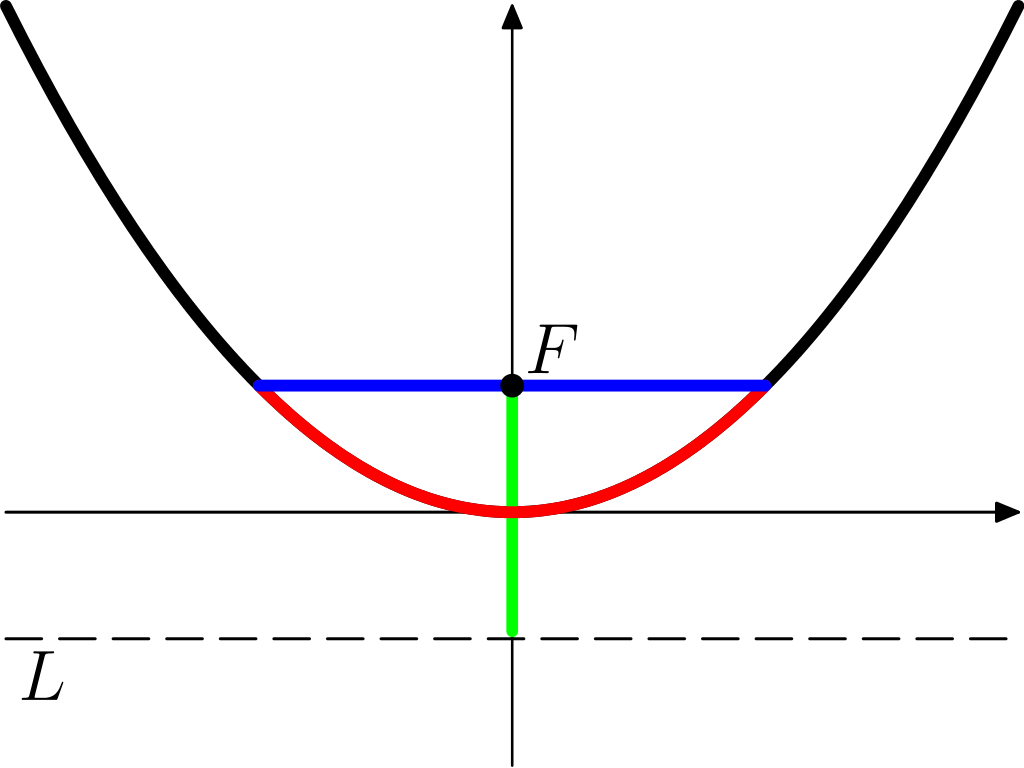
\includegraphics[width=.2\textwidth,center]{upc.png}
    \caption{The universal parabolic constant is the red length divided by the green length.}
\end{figure}

\section{Properties}
\onehalfspacing
\newline
\begin{itemize}
  \item P is an irrational number.
  \item It is also a transcendental number.
\end{itemize}





\newpage


\chapter{Interview}
\section{Criteria for the selection of the interviewee }
\newline

\begin{itemize}
  \item The interviewee should have experience in dealing with constants such as Universal Parabolic Constant.
  \item Since Universal Parabolic Constant is being applied in various contexts, Interviewee can be from Mathematics or Physics background.
\end{itemize}



\section{Interviewee}
\newline Name    : Srividya Murugan
\newline Email : srividya92.sv@gmail.com
\newline Background : She has done Master's in Applied Mathematics.

\newenvironment{qanda}{\setlength{\parindent}{0pt}}{\bigskip}
\newcommand{\Q}{\bigskip\bfseries Q: }
\newcommand{\A}{\par\textbf{A:} \normalfont}
 

\section{Questions \& Answers}
\begin{qanda}
 
\Q How long have you been working with constants?
\A 3 years

\Q Why do we need constants in Math?
\A Mathematical Constants have the value which is fixed by a definition. It will be used across multiple mathematical problem.

\Q How is Universal Parabolic Constant applied?
\A It is not widely used. But it is used in specific complex applications. Eg. Parabolic Bridge


\Q How is Universal Parabolic Constant applied?
\A It is not widely used. But it is used in specific complex applications. Eg. Parabolic Bridge (Physics).

\Q What is the constant's value?
\A It is a fixed value that can be derived from the below equation.

\begin{equation}
P = \ln(1+\sqrt{2})+\sqrt{2} = 2.29558714939
\end{equation}

\Q How often you use this constant in your research area?
\A I use this constant in my study frequently.

\Q Do you use calculator often?
\A Yes.

\Q Do you find it hard to use the irrational numbers while using the calculator? 
\A Yes. It is quite difficult to type irrational numbers with the other numbers. It is not easy to double check.

\Q  Will integrating this constant in the calculator make your calculation easy? 
\A Yes. 

\Q  Do you want to display the symbol or the irrational number in the calculator?
\A  Symbol would be fine.






\section{Analysis}

It is obvious that Mathematicians need an efficient way to use these constants in the calculator. They find it hard to type irrational numbers in the calculator since they use these numbers often in their study. They need these constants in the calculator which would make their calculation easy. 



\end{qanda}
\newpage
\chapter{User Persona}
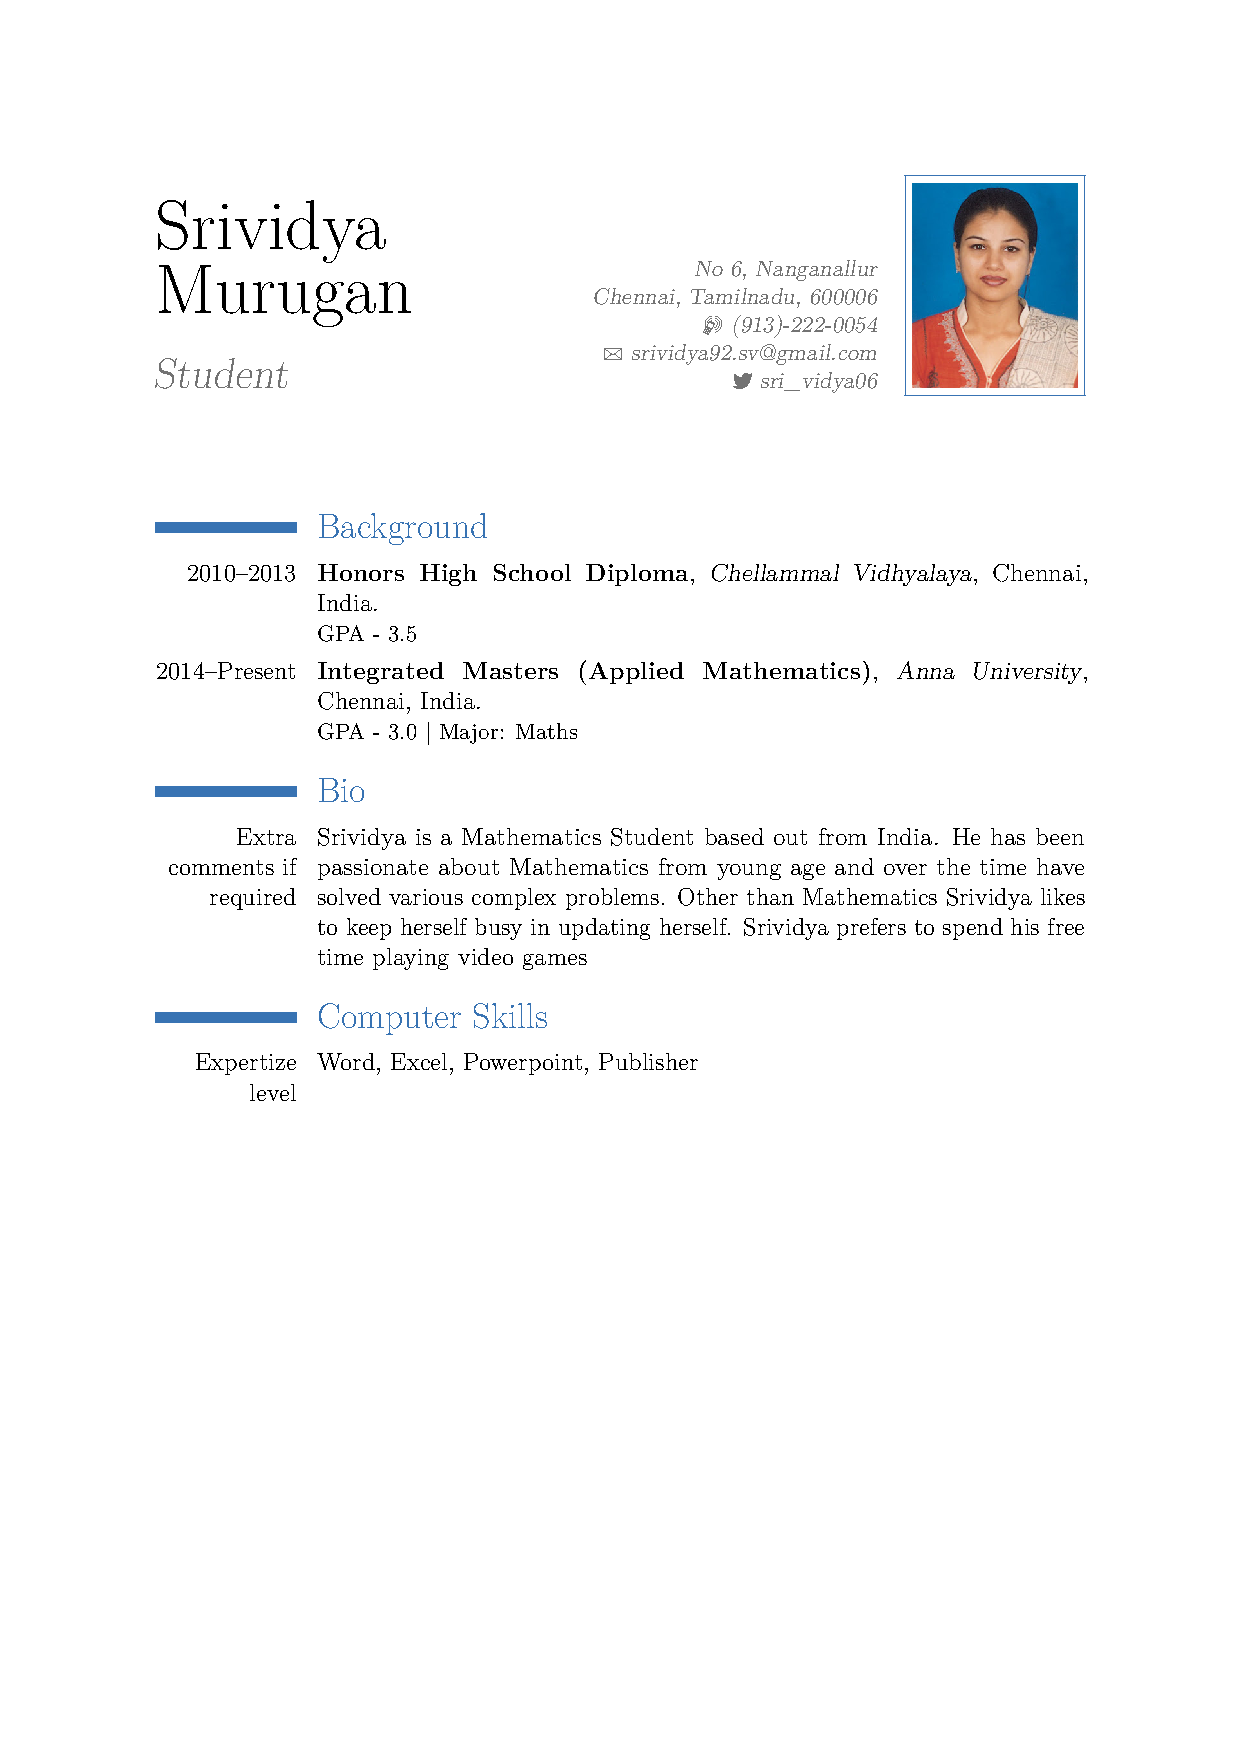
\includepdf[pages=1]{Persona.pdf}
\includepdf[pages=2]{Persona.pdf}



\newpage
\chapter{Problem Domain}
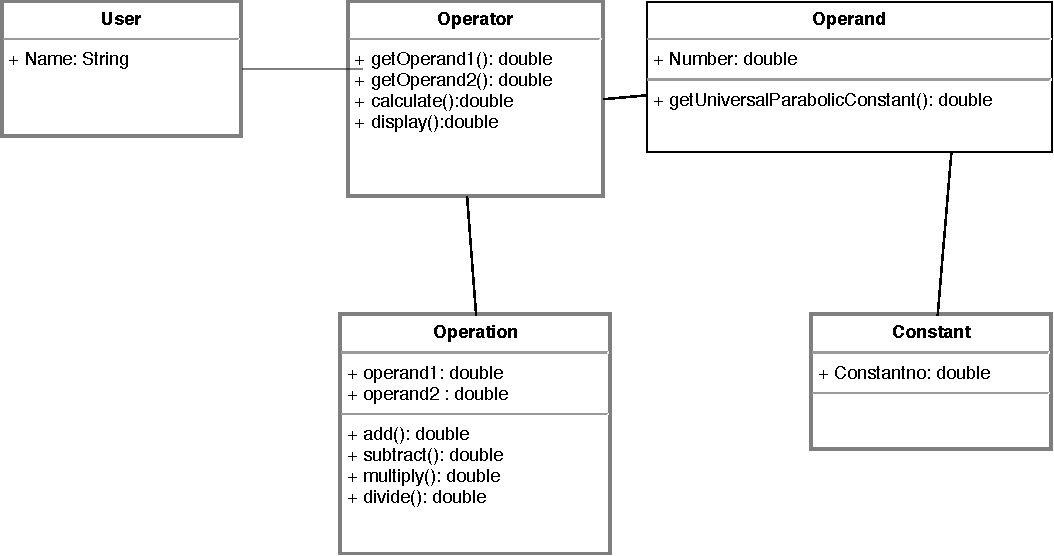
\includepdf[pages=1]{domain.pdf}
\newpage
\section{Description}
A calculator has 4 operators which are Add, Subtract, Multiply, Divide.
\subsection{User}
A user is a person who is using the calculator.
\subsection{Operator}
A user can use an operator to perform his calculation.\newline

\subsection{Operand}
Operand class shall be used to get all the irrational number. 
\subsection{Operation}
Addition, subtraction, multiplication and division are performed by this class.

\subsection{Constant}This class is for the Universal parabolic constant.
\chapter{Activity Diagram}
\section{Description}
The user enters the operands and the operator. Here, we have considered universal parabolic constant as the second operand. Once the user clicks equal operator, corresponding operations will be performed on operands.

\begin{itemize}
    \item If the user selects the "Add" function then the first and constant value will be added
    \item If the user selects the "Subtract" function then the constant will be subtracted from the first number.
    \item If the user selects the "Multiply" function then the first and constant value will be Multiplied
    \item If the user selects the "Divide" function then the first will be divided by the constant.
\end{itemize}
Finally, results will be displayed.

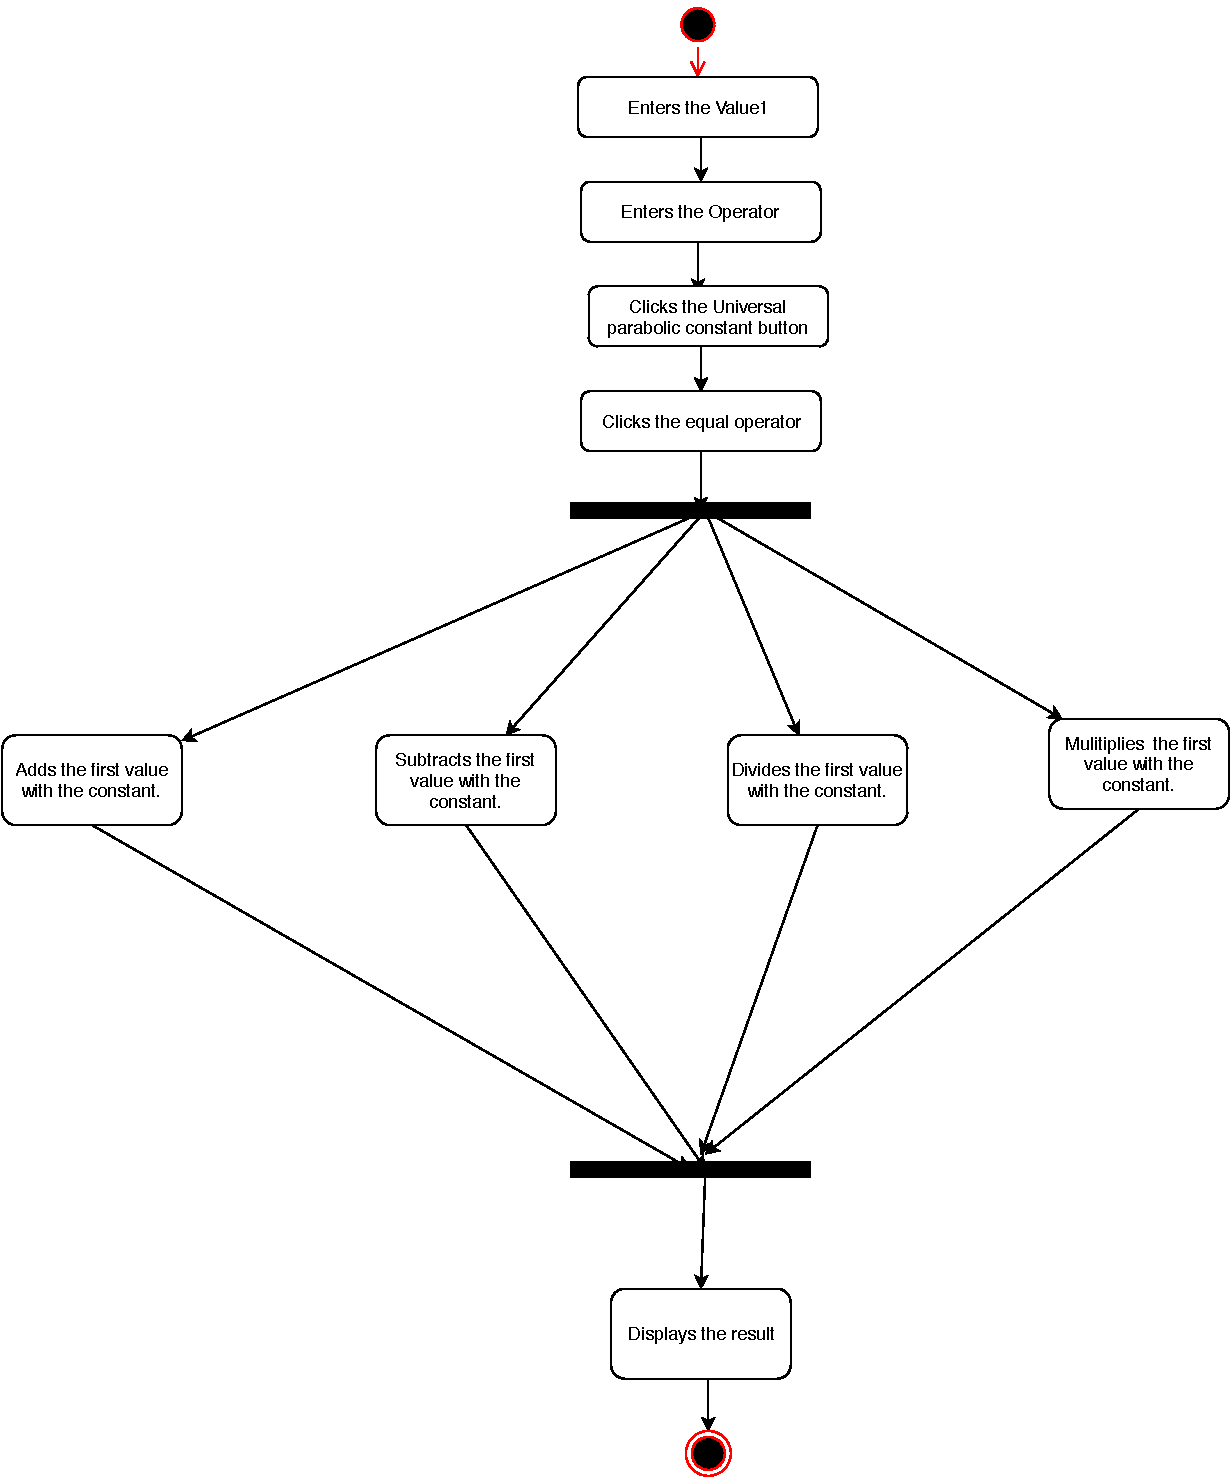
\includepdf[pages=1]{Activity.pdf}
\newpage
\newpage
\chapter{Use Case Diagram}

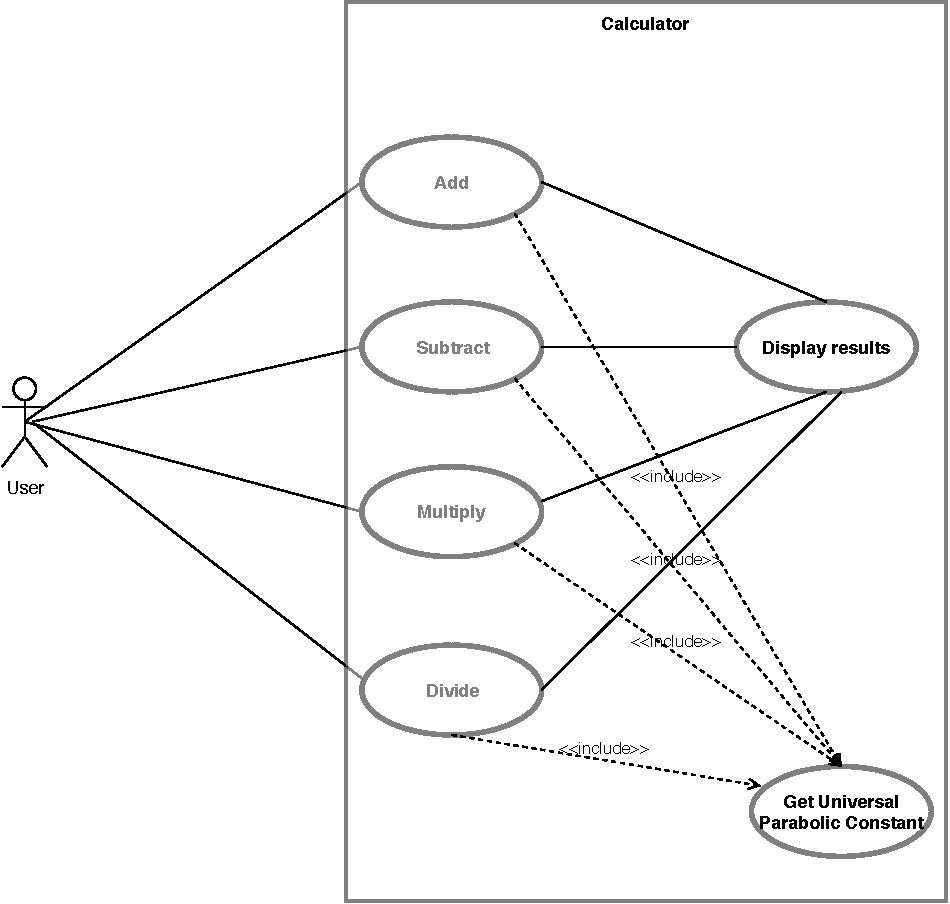
\includepdf[pages=1]{usecase.pdf}
\section{Description}
\begin{itemize}
    \item The goal of the "Add" Use case is to add the two numbers. 
    \item The goal of the "Sub" Use case is to subtract the two numbers. 
    \item The goal of the "Multiply" Use case is to Multiply the two numbers. 
    \item The goal of the "Divide" Use case is to divide the two numbers.
    \item The goal of the "Get Universal Parabolic Constant" Use case is to get the constant.
\end{itemize}
Finally, the goal of the "Display" use case is to display the results of the calculation.

\bibliographystyle{plain}
\bibliography{references}
\end{document}